%%%%%%%%%%%%%%%%%%%%%%%%%%%%%% User specified LaTeX commands.
% report_31_01_2018.tex
% Omkar H. Ramachandran
% omkar.ramachandran@colorado.edu
%
% Documentation for hemispheric dependence in the Fermi Pass 8 data
%

\documentclass[english]{article}
\usepackage[T1]{fontenc}
\usepackage[latin9]{inputenc}
\usepackage{geometry}
\geometry{verbose,tmargin=1.5in,bmargin=1.5in,lmargin=1.5in,rmargin=1.5in}
\usepackage{babel}
\newcommand{\GeV}{\,{\rm GeV}}
\newcommand{\MHz}{\,{\rm MHz}}
\usepackage{graphicx}
\graphicspath{{./plots/}}
\usepackage{hyperref}
\usepackage{listings}
\usepackage{color}
\usepackage{float}

\lstdefinestyle{custompy}{
  belowcaptionskip=1\baselineskip,
  breaklines=true,
  frame=L,
  xleftmargin=\parindent,
  language=Python,
  showstringspaces=false,
  basicstyle=\footnotesize\ttfamily,
  keywordstyle=\bfseries\color{green},
  commentstyle=\itshape\color{red},
  identifierstyle=\color{black},
  stringstyle=\color{blue},
}

\lstset{escapechar=@,style=custompy}

\begin{document}

\title{Prelab 6 : Optical Communication Link}

\author{Omkar H. Ramachandran}
\maketitle

\section{Room Light Photometer}

\subsection{Estimate $S_{\lambda}$}

From the chart provided in the Lab manual, we see that $550\ nm$
corresponds roughly to an $RSR$ of $0.65$. Thus if the peak sensitivity
is at $10\ \mu A/(mW/cm^{2})$, then the $RSR$ at $550\ nm$ is $6.5\ \mu A/(mW/cm^{2})$

\subsubsection*{Does $550\ nm$ make sense?}

Yes, assuming that white light is purely a combination of the seven
colours, we would expect the mean to be somewhere in the middle of
the visible band. The wavelength of blue light is in the vicinity
of $700\ nm$ and red at $400\ nm$. Thus, it makes sense for the
mean to sit at $550\ nm$

\subsection{How much light falls on the PD204?}

According the device manual, the upper surface has a diameter of $3\ mm$.
Thus, the surface area that is facing the bulb is
\[
A=\pi\left(\frac{3}{2}\times10^{-1}\right)^{2}=\pi\frac{9}{4}\frac{1}{100}=0.0706\ cm^{2}
\]
Assuming that the light was on the ceiling, consider a source placed
far enough away that the light rays on reaching the photodiode are
largely parallel. Further, assume that the tube is about a half a
metre long and $10\ cm$ wide. Thus, the overall area is $500\ cm^{2}$.
Assuming that diffraction effects are minimal (reasonably considering
that the width of the tube is much larger than the mean wavelength
$10\ cm\gg\lambda=5.5\times10^{-5}\ cm$), the ratio of areas is simply
\[
\frac{0.0706}{500}=14.12\times10^{-5}
\]
Thus, if the total power output facing the diode is $2\ W$, then
the power incident on the diode is $0.28\ mW/cm^{2}$

\subsection{State three key assumptions of your model}
\begin{enumerate}
\item I'm assuming that the source is a focused beam that is placed far
enough away that the light rays incident on the photodiode are largely
parallel
\item I've assumed that the width of the source container is much larger
than the wavelength of the incident light ray, so as to eliminate
diffraction effects
\item I've assumed that there are no fluctuations in the power output of
the bulb
\end{enumerate}

\section{Trans-Impedance Amplifier}

\subsection{Choose $R_{F}$}

We know that $I=S_{\lambda}N$ and
\[
G=\frac{V_{out}}{I_{in}}=-R_{f}
\]
Thus,
\[
\frac{V_{out}}{S_{\lambda}N}=-R_{f}
\]
We want $V_{out}=10$ for $S_{\lambda}=6.5\ \mu A/\left(mW/cm^{2}\right)$
and $N=1.0$. Thus,
\[
R_{f}=\frac{10}{6.5\times10^{-6}}=1.53\times10^{6}\ \Omega=1.53\ M\Omega
\]

\subsection{What is $f_{B}$ for a given capacitance?}

\[
f_{B}=\frac{1}{2\pi R_{F}C_{F}}
\]
Plugging in $C_{F}=10^{-11}\ F$, we get
\[
f_{B}=\frac{1}{2\pi\times1.53\times10^{-5}}=10402.2\ Hz
\]

\subsection{What are the voltages at various leads?}

When there is no current flowing through the photodiode, the voltages
at the two input terminals is identically zero, which implies that
the signal at the output is also zero.

\subsection{What is the diode is forward biased?}

If the diode is forward biased, the voltage input is $0.6\ V$, implying
that the output will hit the power rail's maximum allowed voltage
- in our case $15\ V$

\section{Optical Communication Link}

\[
N=\frac{1}{683y\left(\lambda\right)}\frac{1}{R^{2}}\;J\left(mcd\right)
\]

\subsection{$J=20\ mA$}

\begin{figure}
\begin{centering}
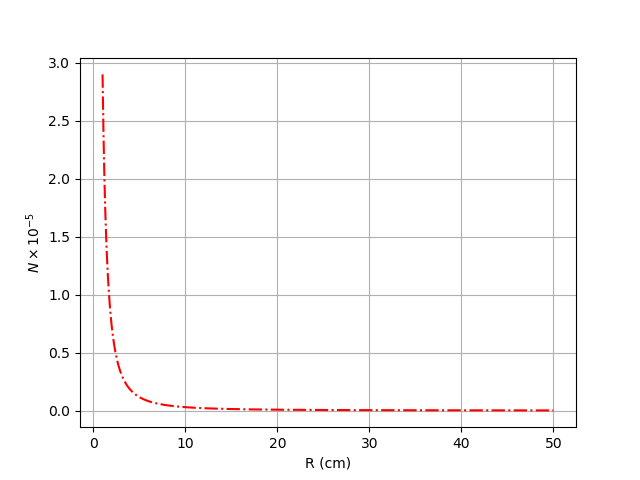
\includegraphics[scale=0.5]{plots/NvR}
\par\end{centering}
\caption{Plot of $N$ vs $R$ for $J\sim20\ mA$ and $\lambda=550\ nm$}
\end{figure}
We end up with 
\[
N=\frac{20\times10^{-3}}{683R^{2}}=\frac{2.9\times10^{-5}}{R^{2}}
\]
since $y\left(550\ nm\right)\sim1$ from the plot shown in the manual.
Figure 1 shows the trend of $N$ vs $R$ for values between $1$ and
$50\ cm$

\subsection{Trend of expected $V_{out}$}

\begin{figure}
\begin{centering}
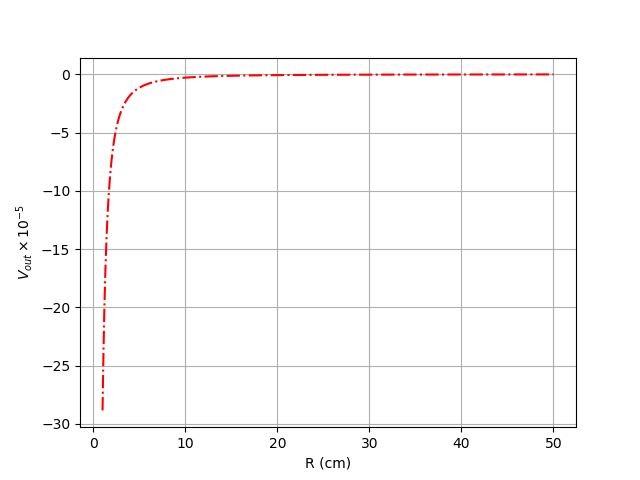
\includegraphics[scale=0.5]{plots/VoutvR}
\par\end{centering}
\caption{Plot of $V_{out}$ vs $R$ for $J\sim20\ mA$ and $\lambda=550\ nm$}
\end{figure}

\[
G=\frac{V_{out}}{I_{in}}=-R_{F}
\]
Thus,
\[
V_{out}=-R_{f}S_{\lambda}N=-1.53\times10^{6}\times6.5\times10^{-6}\frac{2.9\times10^{-5}}{R^{2}}=-\frac{28.84\times10^{-5}}{R^{2}}
\]

\subsection{Compute the required series resistance}

We know that the LED itself drops $1.9\ V$ for $20\ mA$ of current.
Thus,
\[
R_{LED}=\frac{1.9}{20\times10^{-3}}=95\ \Omega
\]
Further, we assume that $R_{internal}=50\ \Omega$. We need a series
resistance $R_{s}$ such that at the high output level:
\[
\frac{10}{R_{LED}+R_{internal}+R_{s}}=\frac{10}{95+50+R_{s}}=20\ mA
\]
Thus,
\[
145+R_{s}=\frac{10}{20\times10^{-3}}=500
\]
\[
R_{s}=355\ \Omega
\]

\section{Lab Activities}
\begin{enumerate}
\item Step 4d where we measure the frequency limitations seems to be the
most challanging. Unlike in previous experments, we're actually measuring
the rise time of the square wave itself - I think - which might be
tricky. Getting rid of background light will also be tricky.
\item Are the sources that we're going to use premeasured - or is there
some way in which we can independently calibrate their intensity?
If we get stuck with a faulty diode, I'd like a way to confirm measurements.
\end{enumerate}

\end{document}
